%Old Version from Greg. Greg, this slide is changed substantially, please take a look.
%% begin module power-functions-def
%\begin{frame}
%\frametitle{Power Functions}
%\begin{definition}[Power Function]
%A power function is a function of the form
%\[
%f(x) = x^a,
%\]
%where $a$ is a fixed real number.
%\end{definition}
%\uncover<2->{
%If $a$ is a positive integer like $1, 2, 3, \ldots$ then $x^a$ is a polynomial.

%\only<handout:-2| -2>{%
%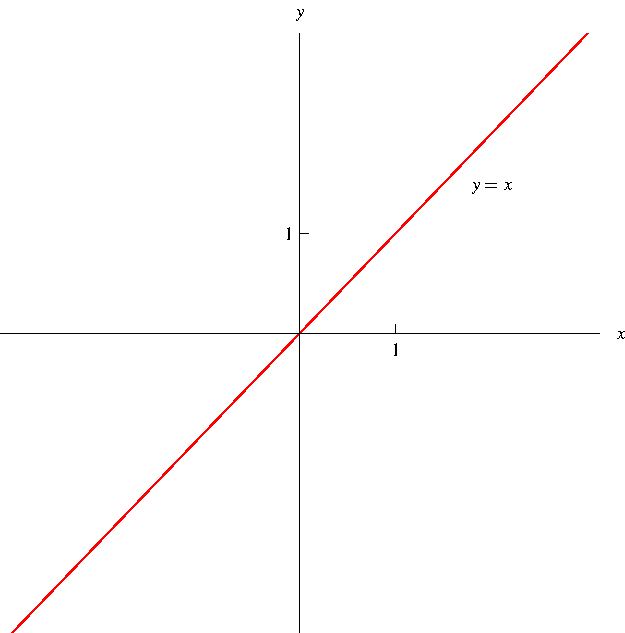
\includegraphics[height=4cm]{precalculus/pictures/01-02-x.pdf}%
%}%
%\only<handout:3| 3>{%
%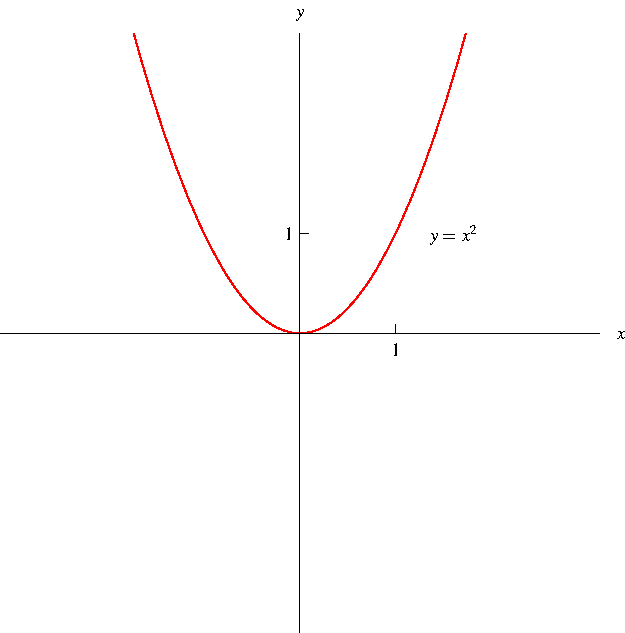
\includegraphics[height=4cm]{precalculus/pictures/01-02-xsquared.pdf}%
%}%
%\only<handout:4| 4>{%
%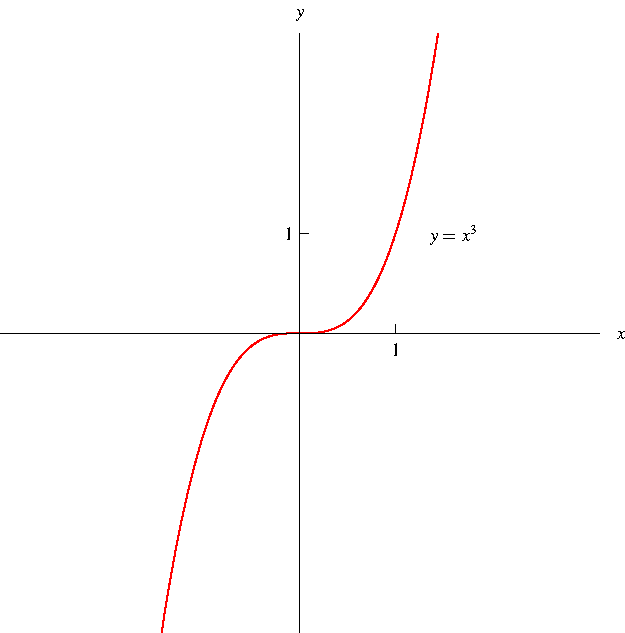
\includegraphics[height=4cm]{precalculus/pictures/01-02-xcubed.pdf}%
%}%
%\only<handout:5| 5>{%
%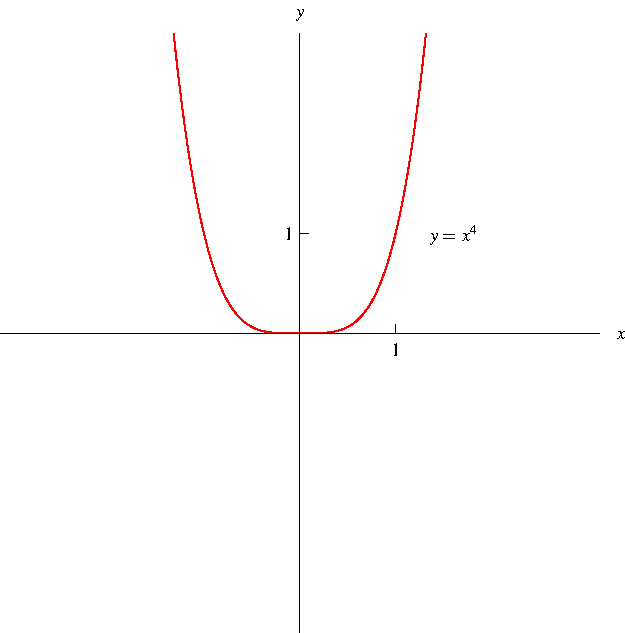
\includegraphics[height=4cm]{precalculus/pictures/01-02-xfourth.pdf}%
%}%
%\only<handout:6| 6>{%
%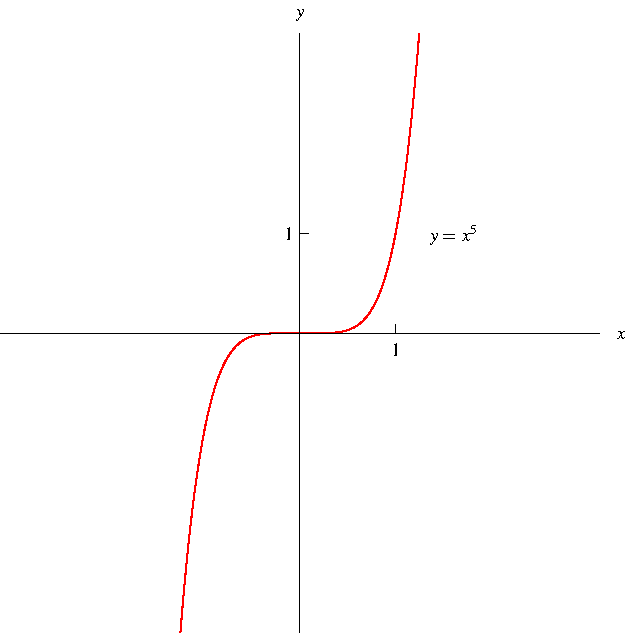
\includegraphics[height=4cm]{precalculus/pictures/01-02-xfifth.pdf}
%}%
%}%
%\end{frame}
%% end module power-functions-def

% begin module power-functions-def
\begin{frame}[t]
\frametitle{Power Functions}
\begin{definition}[Power Function]
Let $x>0$, $a$ - arbitrary real number. The power function is defined as
\[
f(x) \uncover<4->{\alertNoH{ 4}{=e^{a\ln x} } }= \alertNoH{2}{x}^{\alertNoH{3}{a}} \quad .
\]
\uncover<2->{$x$ = \alertNoH{2}{base}. } \uncover<3->{$a$ = \alertNoH{3}{exponent} or \alertNoH{3}{power}. }
\uncover<4->{\alertNoH{ 4}{First equality = one of ways to define for non-integer $a$ (we study $\ln x$, $e^x$ later). } }
\end{definition}
\begin{tabular}{@{}l}
\uncover<5->{
If $a$ - positive integer ($1, 2, 3, \ldots$) \\
then $x^a$ = polynomial function.
}\\
\uncover<5->{
$x^{n}    =\underbrace{x\dots x }_{n~\mathrm{times}}$ when $n$-integer. \\

$\begin{array}{rcl}
\alertNoH{12}{(x^{a})^b}&=&\fcAnswer{13}{x^{ab}}  \\
\alertNoH{14}{(xy)^b}   &=&\fcAnswer{15}{ x^by^b}\\
\alertNoH{16}{x^{a+b}}  &=&\fcAnswer{17}{x^ax^b } \\
\alertNoH{18}{x^{-a}}   &=&\fcAnswer{19}{\frac{1}{x^a}}
\end{array}
$\\
~\\~\\~\\~\\~\\~\\~\\
}
\end{tabular}
\uncover<6->{
\psset{xunit=0.38cm,yunit=0.38cm}
\begin{pspicture}(-5,-5)(5.4,5.2)
\psaxes[labels=none]{<->}(0,0)(-5,-5)(5,5)
\tiny
\rput[r](0,5){\tiny{$y$}}
\rput[l](5,0){\tiny{$x$}}
\only<handout:1|7>{
\psplot[linecolor=red]{-5}{5}{ x 1 exp }
\rput( 3, 1){$y=x^{\phantom{1}}$}
} %only
\only<handout:2|8>{
\psplot[linecolor=red]{-2.23}{2.23}{ x 2 exp }
\rput( 3, 1){$y=x^2$}
}
\only<handout:3|9>{
\psplot[linecolor=red]{-1.7}{1.7}{ x 3 exp }
\rput( 3, 1){$y=x^3$}
}
\only<handout:4|10>{
\psplot[linecolor=red]{-1.49}{1.49}{ x 4 exp }
\rput( 3, 1){$y=x^4$}
}
\only<handout:5|11->{
\psplot[linecolor=red]{-1.37}{1.37}{ x 5 exp }
\rput( 3, 1){$y=x^5$}
}
\end{pspicture}
\uncover<handout:5|11->{}
%\only<handout:-2| -2>{%
%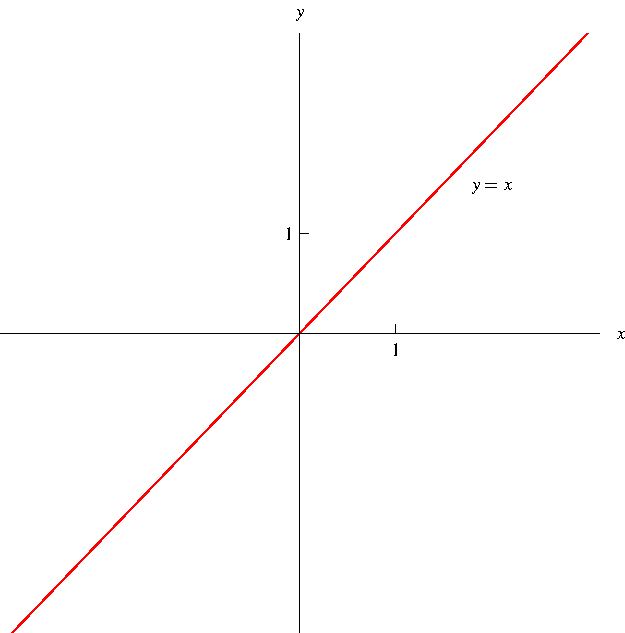
\includegraphics[height=4cm]{precalculus/pictures/01-02-x.pdf}%
%}%
%\only<handout:3| 3>{%
%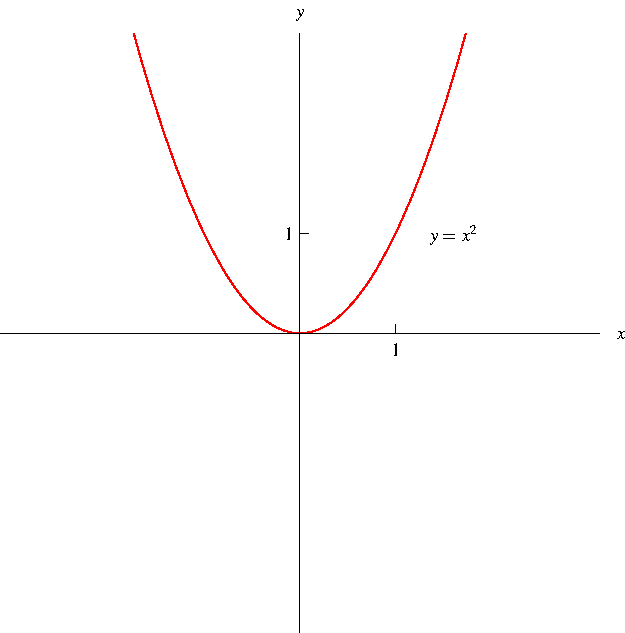
\includegraphics[height=4cm]{precalculus/pictures/01-02-xsquared.pdf}%
%}%
%\only<handout:4| 4>{%
%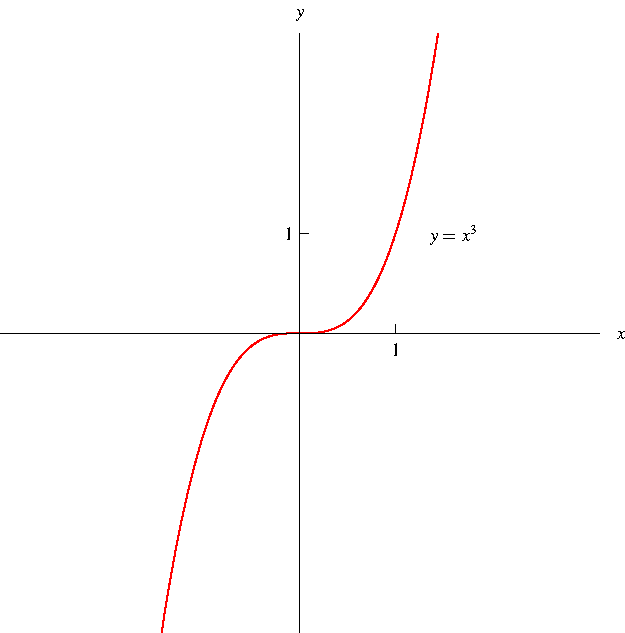
\includegraphics[height=4cm]{precalculus/pictures/01-02-xcubed.pdf}%
%}%
%\only<handout:5| 5>{%
%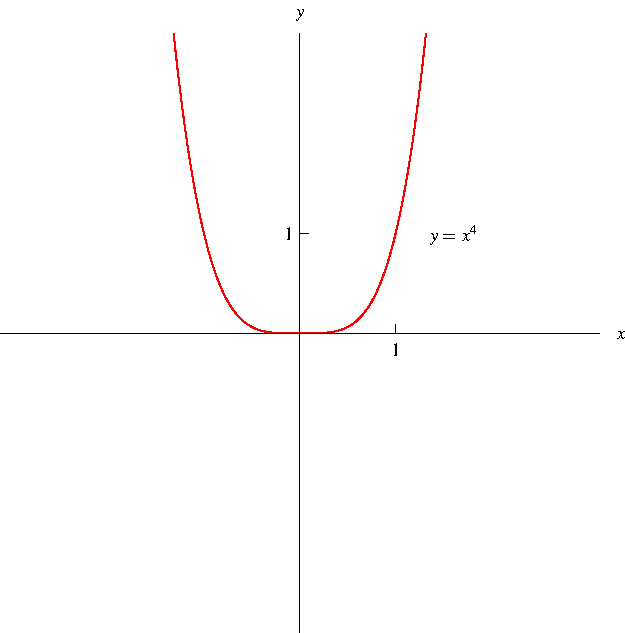
\includegraphics[height=4cm]{precalculus/pictures/01-02-xfourth.pdf}%
%}%
%\only<handout:6| 6>{%
%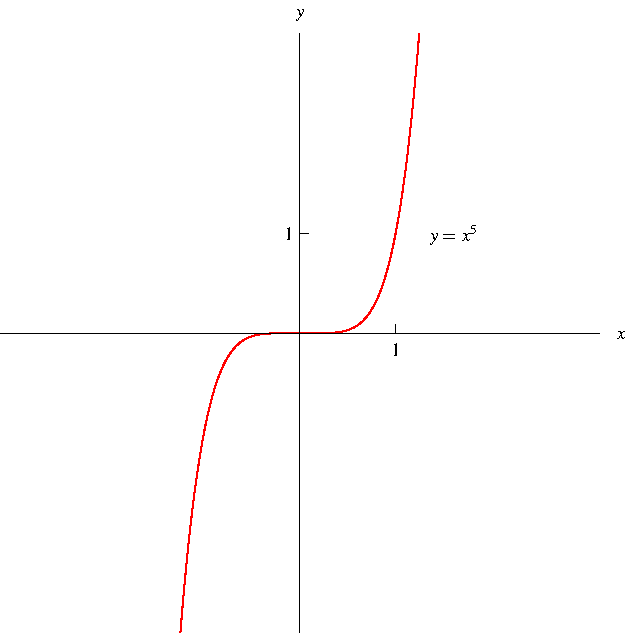
\includegraphics[height=4cm]{precalculus/pictures/01-02-xfifth.pdf}
%}%
}
\end{frame}
% end module power-functions-def
